% PREAMBLE
\documentclass[11pt]{amsart}
\usepackage[T1]{fontenc}
\usepackage{lmodern}
\usepackage{microtype}
\usepackage{amsmath,amssymb}
\usepackage{mathtools}
\usepackage{graphicx}
\usepackage{booktabs}
\usepackage{tikz}
\usepackage[colorlinks=true,linkcolor=blue!45!black,citecolor=blue!45!black,urlcolor=blue!45!black]{hyperref}
\usepackage[capitalize]{cleveref}

\newtheorem{theorem}{Theorem}[section]
\newtheorem{proposition}[theorem]{Proposition}
\newtheorem{lemma}[theorem]{Lemma}
\newtheorem{corollary}[theorem]{Corollary}
\newtheorem{conjecture}[theorem]{Conjecture}
\theoremstyle{definition}
\newtheorem{definition}[theorem]{Definition}
\newtheorem{fact}[theorem]{Fact}
\theoremstyle{remark}
\newtheorem{remark}[theorem]{Remark}

\title[Parity Carpets Correlate by gcd]{Parity Carpets Correlate by gcd: Four Exact Laws for a Square-Wave Stack}
\author{Carlo Mitchener}
\email{carlo.mitchener@gmail.com}
\date{2026-08-23}

% PAPER
\begin{document}

\begin{abstract}
Cut a square into an odd number of equal strips each way and ink every cell whose two strip numbers are both odd. Two such pictures at different scales overlap by an amount fixed by the greatest common divisor of the scales, and that amount is exact. We prove the master integral behind it, derive the exact correlation law for each of the four fields the parity rule generates, and show that all four vanish precisely when the scales are coprime. So an odd number above one is prime exactly when its picture is uncorrelated with every picture before it: a portrait of coprimality, not a primality test. Two ray laws are proved alongside, and two boundaries: the exactness fails in a hexagonal section, and the stack's brightness carries no M\"obius information.
\end{abstract}

\maketitle

\section{Introduction}
\label{sec:intro}

\begin{figure}[!ht]
\centering
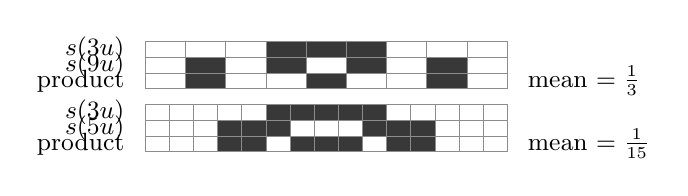
\begin{tikzpicture}[x=46mm,y=2.0mm]
\foreach \i in {3,4,5} \fill[black!78] ({\i/9},6) rectangle ({(\i+1)/9},7);
\foreach \i in {0,...,8} \draw[black!45,line width=0.2pt] ({\i/9},6) rectangle ({(\i+1)/9},7);
\foreach \i in {1,3,5,7} \fill[black!78] ({\i/9},5) rectangle ({(\i+1)/9},6);
\foreach \i in {0,...,8} \draw[black!45,line width=0.2pt] ({\i/9},5) rectangle ({(\i+1)/9},6);
\foreach \i in {1,4,7} \fill[black!78] ({\i/9},4) rectangle ({(\i+1)/9},5);
\foreach \i in {0,...,8} \draw[black!45,line width=0.2pt] ({\i/9},4) rectangle ({(\i+1)/9},5);
\foreach \i in {5,6,7,8,9} \fill[black!78] ({\i/15},2) rectangle ({(\i+1)/15},3);
\foreach \i in {0,...,14} \draw[black!45,line width=0.2pt] ({\i/15},2) rectangle ({(\i+1)/15},3);
\foreach \i in {3,4,5,9,10,11} \fill[black!78] ({\i/15},1) rectangle ({(\i+1)/15},2);
\foreach \i in {0,...,14} \draw[black!45,line width=0.2pt] ({\i/15},1) rectangle ({(\i+1)/15},2);
\foreach \i in {3,4,6,7,8,10,11} \fill[black!78] ({\i/15},0) rectangle ({(\i+1)/15},1);
\foreach \i in {0,...,14} \draw[black!45,line width=0.2pt] ({\i/15},0) rectangle ({(\i+1)/15},1);
\node[anchor=east,font=\small] at (-0.03,6.5) {$s(3u)$};
\node[anchor=east,font=\small] at (-0.03,5.5) {$s(9u)$};
\node[anchor=east,font=\small] at (-0.03,4.5) {product};
\node[anchor=east,font=\small] at (-0.03,2.5) {$s(3u)$};
\node[anchor=east,font=\small] at (-0.03,1.5) {$s(5u)$};
\node[anchor=east,font=\small] at (-0.03,0.5) {product};
\node[anchor=west,font=\small] at (1.03,4.5) {mean $=\tfrac13$};
\node[anchor=west,font=\small] at (1.03,0.5) {mean $=\tfrac{1}{15}$};
\end{tikzpicture}
\caption{Two parity waves and their product; a cell is dark where the wave is $-1$. The product's mean is exactly $\gcd(m,n)^2/(mn)$: one third for $(3,9)$, one fifteenth for the coprime $(3,5)$.}
\label{fig:overlap}
\end{figure}

Here is a picture anyone can draw. Fix an odd number $n$, cut the unit square into $n$ columns and $n$ rows numbered from zero, and shade a cell when both its numbers are odd. Draw a second sheet at a different odd $n$ and hold the two up to the light: how much do they agree? The answer is one exact number. With $g=\gcd(m,n)$ for the two scales, the correlation of the sheets has $g$ in its numerator and is \emph{exactly zero} when $g=1$ -- not small, not zero to five decimals, zero.

\subsection{The master integral, and what is classical about it}
\label{sec:prior}

Everything rests on one integral. With $s(x)=(-1)^{\lfloor x\rfloor}$ the square wave of period $2$, for all positive integers $m,n$ with $g=\gcd(m,n)$,
\[
\int_0^1 s(mu)\,s(nu)\,du=\frac{g^2}{mn}\ \ \text{if $m/g$ and $n/g$ are both odd},\qquad 0\ \text{otherwise.}
\]
\Cref{fig:overlap} is that statement drawn twice.

This identity has a famous sibling. With $((x))$ the sawtooth $x-\lfloor x\rfloor-\tfrac12$ (and $((x))=0$ at integers),
\[
\int_0^1 ((mx))\,((nx))\,dx=\frac{\gcd(m,n)^2}{12\,mn},
\]
which is the two-fold Franel integral, standard in the literature of Dedekind sums \cite{apostol}, the base case of the family whose four-fold generalisation was conjectured by McIntosh and proved recently \cite{mcintosh}, and the computational heart of the Franel-Landau reformulation of the Riemann hypothesis. Our master integral is the same computation with the sawtooth's full harmonic comb replaced by the square wave's odd-only comb, by the same Parseval argument. That substitution is exactly where the hypothesis ``$m/g$ and $n/g$ both odd'' comes from, and why the constant is $1$ rather than $1/12$. A referee should read \cref{thm:master} as a gcd-sum evaluation of a routine kind, not as a new theorem; the classical identity is re-verified alongside ours in \texttt{scripts/verify.py}.

The increment this paper offers is narrower and, we think, more honest to state plainly. First, exactness: the author's own earlier and unpublished working notes on stacked designs already recorded that the cross-layer correlation is about zero at $\gcd=1$ and that it tracks $\gcd^2/(mn)$; what is proved here is that it is \emph{exactly} zero, with closed forms for all four fields and with the coprimality criterion as an identity rather than an observation. Second, the ray laws: the two-adic criterion that a line through the origin of slope $q/p$ carries signal if and only if $p$ and $q$ are both odd. Third, the negative results, which we regard as the most useful part: the failure in the hexagonal section, and the M\"obius refutation. The prime corollary itself claims no novelty at all -- as an algorithm it is trial division with a picture attached.

\subsection{What this paper proves}
\label{sec:roadmap}

The parity of $m/g$ and $n/g$ is not decoration: at $(m,n)=(1,2)$ the integral is $0$ rather than $1/2$, and the unqualified formula fails on $532$ of the $820$ unordered pairs with $m,n\le 40$. From the master integral, four correlation laws drop out, one for each black-and-white field the parity rule generates (\cref{thm:four}), and all four vanish at exactly the same places (\cref{thm:zeroset}). Since an odd composite always has an odd prime factor smaller than itself, the sheet of a composite always echoes a smaller sheet and the sheet of a prime never does (\cref{cor:detector}). The pictures see coprimality; primality is what coprimality against everything smaller happens to mean.

The paper also proves two exact ray laws for the stacked picture (\cref{thm:ray}, \cref{prop:origin}), gives the stack's variance exactly, as a finite rational sum (\cref{prop:variance}), and then marks two boundaries, because a result is only as valuable as the map of where it stops. The plane rule that makes all of this work has a nonzero pair term in its harmonic expansion; the analogous rule in space has none, and with it goes the mechanism (\cref{prop:space}). And the brightness of the stacked picture, tempting as it looks, contains no M\"obius information whatsoever (\cref{prop:brightness}); no Riemann-hypothesis criterion can be read off it.

\section{Definitions}
\label{sec:defs}

\begin{definition}
\label{def:wave}
$s(x)=(-1)^{\lfloor x\rfloor}$ is the square wave of period $2$, and $\chi_n(u)=\mathbf 1[\lfloor nu\rfloor\text{ odd}]=\tfrac12\bigl(1-s(nu)\bigr)$ is the odd-strip indicator at scale $n$. All integrals are over $u\in[0,1)$ or $(u,v)\in[0,1)^2$ with Lebesgue measure, and $\langle\cdot\rangle$ denotes the mean.
\end{definition}

\begin{definition}
\label{def:fields}
For odd $n\ge1$ the parity rule generates four $\{0,1\}$-valued fields on the unit square:
\[
\mathrm{T}_n(u,v)=\chi_n(u),\qquad
\mathrm{C}_n(u,v)=\chi_n(u)\chi_n(v),
\]
\[
\mathrm{N}_n(u,v)=\bigl(1-\chi_n(u)\bigr)\bigl(1-\chi_n(v)\bigr),\qquad
\mathrm{V}_n(u,v)=\tfrac12\bigl(1+s(nu)s(nv)\bigr).
\]
We call them \emph{tree}, \emph{carpet}, \emph{net} and \emph{void}. The tree depends on one coordinate; the carpet marks cells whose two strip numbers are both odd; the net is its complementary product; the void marks cells whose two strip numbers have the same parity.
\end{definition}

The sheet of \cref{sec:intro} is the carpet. Printing it the other way round -- inking every cell \emph{except} those with both indices odd -- gives the field $1-\mathrm{C}_n$, and correlation is invariant under $X\mapsto1-X$ applied to both arguments, so every statement below about $\mathrm{C}$ holds verbatim for that picture too. Of the four, $\mathrm{C}$, $\mathrm{N}$ and $\mathrm{V}$ are the three non-constant fields one can build from the pair $(\chi_n(u),\chi_n(v))$ that respect the symmetry $u\leftrightarrow v$, counted up to complementation: as functions of two bits they are AND, NOR and XNOR, and the remaining three symmetric non-constant functions NAND, OR and XOR are their complements. The tree $\mathrm{T}$ is not symmetric at all -- it reads one coordinate and ignores the other -- and is kept because it is the simplest law of the family.

\begin{definition}
\label{def:corr}
For fields $X,Y$ on the unit square, $\operatorname{Cov}(X,Y)=\langle XY\rangle-\langle X\rangle\langle Y\rangle$ and $r(X,Y)=\operatorname{Cov}(X,Y)/\sqrt{\operatorname{Var}(X)\operatorname{Var}(Y)}$. The \emph{stack} of the first $L$ odd scales is $\frac1L\sum_{n\in S}\mathrm{C}_n$ with $S=\{1,3,\dots,2L-1\}$.
\end{definition}

Because each field is $\{0,1\}$-valued, $r=0$ is more than decorrelation: at a uniformly random point of the square the two values are then independent Bernoulli random variables. The fields themselves are deterministic; the independence is of the two readings taken at one random point, and we never claim more.

\section{Results}
\label{sec:results}

\begin{theorem}[master integral]
\label{thm:master}
Let $m,n\ge1$ be integers, $g=\gcd(m,n)$, $m'=m/g$, $n'=n/g$. Then
\[
\int_0^1 s(mu)\,s(nu)\,du=
\begin{cases}
\dfrac{g^2}{mn}, & m'\text{ and }n'\text{ both odd},\\[2mm]
0, & \text{otherwise.}
\end{cases}
\]
\end{theorem}

\begin{corollary}
\label{cor:odd}
For odd $m,n$ the integral is $g^2/(mn)$; in particular $\langle s(nu)\rangle=1/n$ and $\langle\chi_n\rangle=\frac{n-1}{2n}$ for odd $n$.
\end{corollary}

The right-hand side is rational, and this is worth a sentence: the square wave's Fourier normalisation contributes $(4/\pi)^2$ and the odd Basel sum $\sum_{k\text{ odd}}k^{-2}=\pi^2/8$ eats it exactly. Every observable in this paper is rational for the same reason. Reporting $\pi$ as a feature of these pictures would be numerology.

\begin{theorem}[four correlation laws]
\label{thm:four}
Let $m,n\ge3$ be odd, $d=\gcd(m,n)$. Then
\[
\operatorname{Cov}(\mathrm{T}_m,\mathrm{T}_n)=\frac{d^2-1}{4mn},\quad
r(\mathrm{T}_m,\mathrm{T}_n)=\frac{d^2-1}{\sqrt{(m^2-1)(n^2-1)}},
\]
\[
\operatorname{Cov}(\mathrm{C}_m,\mathrm{C}_n)=\frac{(d^2-1)\bigl[2(m-1)(n-1)+d^2-1\bigr]}{16m^2n^2},
\]
\[
r(\mathrm{C}_m,\mathrm{C}_n)=\frac{(d^2-1)\bigl[2(m-1)(n-1)+d^2-1\bigr]}{(m-1)(n-1)\sqrt{(3m-1)(m+1)(3n-1)(n+1)}},
\]
\[
\operatorname{Cov}(\mathrm{N}_m,\mathrm{N}_n)=\frac{(d^2-1)\bigl[2(m+1)(n+1)+d^2-1\bigr]}{16m^2n^2},
\]
\[
r(\mathrm{N}_m,\mathrm{N}_n)=\frac{(d^2-1)\bigl[2(m+1)(n+1)+d^2-1\bigr]}{(m+1)(n+1)\sqrt{(3m+1)(m-1)(3n+1)(n-1)}},
\]
\[
\operatorname{Cov}(\mathrm{V}_m,\mathrm{V}_n)=\frac{d^4-1}{4m^2n^2},\qquad
r(\mathrm{V}_m,\mathrm{V}_n)=\frac{d^4-1}{\sqrt{(m^4-1)(n^4-1)}}.
\]
\end{theorem}

The four formulas are different functions and must not be substituted for one another. At $(m,n)=(3,9)$ they read $0.316227766$ for the tree, $0.262950294$ for the net, $0.219264505$ for the carpet and $0.110431526$ for the void: one zero set, four different sizes. The tree law is the simplest and the most quotable, but the picture a reader draws from \cref{sec:intro} is the carpet, and the carpet's law is the third one.

\begin{theorem}[one zero set, and strict positivity off it]
\label{thm:zeroset}
For odd $m,n\ge3$, all four covariances of \cref{thm:four} are $0$ if $\gcd(m,n)=1$ and all four are strictly positive if $\gcd(m,n)>1$. In particular the four fields share one zero set, and $\operatorname{Cov}=0\iff\gcd(m,n)=1$ in each family.
\end{theorem}

\begin{corollary}[the coprimality detector]
\label{cor:detector}
Let $n\ge3$ be odd and let $\mathcal F$ be any one of the four families. Then $n$ is prime if and only if $\operatorname{Cov}(\mathcal F_m,\mathcal F_n)=0$ for every odd $m$ with $3\le m<n$.
\end{corollary}

This is independent of any window: it holds for the infinite family of odd scales, not merely inside some finite stack. A finite stack can only distort it. In a stack of the odd scales up to $55$, for instance, the scales with no echo at all are $19,23,29,31,37,41,43,47,53$, which are the primes above $55/3$; that list is an artefact of the window, since $17$ is dropped only because $51=3\cdot17$ happens to be in the stack. The window statement should never be quoted as the theorem; \cref{cor:detector} is the theorem.

\begin{fact}
\label{fact:separation}
Score each odd $n$ in $3\le n\le199$ by $\max\{r(\mathrm{C}_m,\mathrm{C}_n):m\text{ odd},\,3\le m<n\}$, the score of $n=3$ being $0$ over an empty set. Then all $45$ primes in the range score exactly $0$ and all $54$ composites score strictly positive, with no overlap. The narrowest composite is $n=169=13^2$ at $0.0517383422$; the same $n$ scores $0.0766964989$ in the tree family and $0.0059170562$ in the void family. Checked by \texttt{scripts/verify.py}.
\end{fact}

\begin{remark}
\label{rem:trial}
\Cref{cor:detector} is not a primality test worth running. Deciding it for one $n$ means testing $\gcd(m,n)=1$ for every smaller odd $m$, which is trial division with a picture attached; it detects primes, it does not explain them. Its interest is that a purely geometric question -- do these two drawings agree more than chance? -- has an arithmetic answer with no error term, and that the primes are exactly the drawings that are new. The primes so produced are of course \href{https://oeis.org/A000040}{A000040}.
\end{remark}

\begin{theorem}[the slope-one ray law]
\label{thm:ray}
Let $S=\{1,3,\dots,2L-1\}$ and, for real $c$, let
\[
Q_L(c)=\frac1L\sum_{n\in S}\int_0^1 s(nu)\,s(nu+nc)\,du .
\]
If $c=a/b$ in lowest terms, then
\[
\lim_{L\to\infty}Q_L(a/b)=\frac{(-1)^a}{b^2}\ \ (b\text{ odd}),\qquad
\lim_{L\to\infty}Q_L(a/b)=0\ \ (b\text{ even}),
\]
and the limit is $0$ for irrational $c$.
\end{theorem}

\begin{proposition}[rays through the origin]
\label{prop:origin}
Let $p,q\ge1$ be coprime and $n$ odd. The mean of $s(nu)s(nv)$ along the line $(u,v)=(pw,qw)$, $w\in[0,1)$, equals $1/(pq)$ if $p$ and $q$ are both odd, and $0$ otherwise. The value does not depend on $n$, hence is also the value for every stack.
\end{proposition}

\begin{remark}
\label{rem:notacorr}
The number $1/(pq)$ in \cref{prop:origin} is the master integral of \cref{thm:master} evaluated at the coprime pair $(p,q)$: an \emph{uncentred} mean. It is not the correlation of the sheets $p$ and $q$, which by \cref{thm:zeroset} is exactly $0$. The two quantities are computed by one lemma read two ways, and the temptation to call them the same number should be resisted.
\end{remark}

\begin{remark}
\label{rem:finiteN}
\Cref{thm:ray} is a limit, and a finite stack does not sit on it. In the stack of the $28$ odd scales up to $55$: the $b=7$ ray sits exactly on its limit $-1/49$ (because $28=4\cdot7$ samples the residues evenly); the $b=9$ ray reads $+1/63$ against a limit of $-1/81$, the \emph{wrong sign}; the $b=5$ ray is $10/7$ of its limit; and the $b=6$ ray reads $-1/42$ against a limit of $0$, though $b=2$ is exactly $0$ at every stack size. Any image of a finite stack is therefore an illustration of these laws, not a measurement of them.
\end{remark}

\begin{proposition}[exact stack variance]
\label{prop:variance}
For $S=\{1,3,\dots,2L-1\}$ and the carpet stack $G_L=\frac1L\sum_{n\in S}\mathrm{C}_n$,
\[
\operatorname{Var}(G_L)=\frac1{L^2}\sum_{m,n\in S}\frac{(d^2-1)\bigl[2(m-1)(n-1)+d^2-1\bigr]}{16m^2n^2},\quad d=\gcd(m,n),
\]
an exact rational for every $L$. Its values are $L\cdot\operatorname{Var}=0.21014$ at $L=28$, $0.24516$ at $L=101$ and $0.26400$ at $L=501$.
\end{proposition}

\begin{conjecture}
\label{con:variance}
$\lim_{L\to\infty}L\cdot\operatorname{Var}(G_L)=0.272442\ldots$, and this constant is a combination of two gcd sums rather than a known closed form. Evidence: the exact values $0.21014$, $0.24516$ and $0.26400$ of \cref{prop:variance} climb towards it, and the limit reduces to the two gcd sums
\[
S_2(N)=\sum g^2/(mn),\quad S_4(N)=\sum g^4/(m^2n^2)\quad(m,n\ \text{odd},\ \le N)
\]
as $\lim_{N\to\infty}S_2(N)/(4N)+\lim_{N\to\infty}S_4(N)/(8N)$. The second of these reduces to a single gcd sum,
\begin{gather*}
\lim_{N\to\infty}\frac{S_4(N)}{N}=\frac{16}{31}\cdot\frac{T}{\zeta(5)}=0.5536124372\ldots,\\
T=\sum_{k,l\ \text{odd}}\frac{1}{k^2l^2\max(k,l)}=1.1122336970\ldots,
\end{gather*}
so the second term contributes $0.06920155\ldots$ and the first carries the rest. Failure modes: no closed form is known for $T$, so the constant is \emph{reduced}, not evaluated; the reduction's error term is only measured, at five digits and still drifting; and the finite-$L$ approach is slow enough ($23\%$ short at $L=28$) that agreement at accessible $L$ is weak evidence for any particular closed form. Nothing in this paper depends on this conjecture.
\end{conjecture}

\subsection{Where the exactness stops}
\label{sec:stops}

\begin{proposition}[the space rule has no pair term]
\label{prop:space}
Write $\sigma_i=+1$ if index $i$ is even and $-1$ if it is odd. The plane rule ``ink unless both indices are odd'' has the harmonic expansion
\[
H(\sigma_1,\sigma_2)=\tfrac34+\tfrac{\sigma_1+\sigma_2}{4}-\tfrac{\sigma_1\sigma_2}{4},
\]
while the space rule ``fill if at most one of three indices is odd'' has
\[
F(\sigma_1,\sigma_2,\sigma_3)=\tfrac12+\tfrac{\sigma_1+\sigma_2+\sigma_3}{4}-\tfrac{\sigma_1\sigma_2\sigma_3}{4},
\]
whose three pairwise coefficients are all exactly $0$.
\end{proposition}

The pair term $-\sigma_1\sigma_2/4$ is the entire mechanism of this paper: it is what turns the master integral into a correlation. In space the pair term is absent and a triple product takes its place, so a planar section of the space rule has no reason to inherit any of the exactness -- and it does not.

\begin{remark}
\label{rem:hex}
On rendered hexagonal sections of the space rule at the $28$ scales $1,3,\dots,55$, the $290$ coprime pairs drawn from the $27$ scales $3,\dots,55$ have Pearson correlations with mean $-0.037$ and range $[-0.205,+0.147]$, with $85$ of the $290$ exceeding $0.05$ in absolute value; the corresponding flat-carpet figures on the same raster are mean $-0.0001$ and maximum $0.017$, against exactly $0$ in the continuum. The gcd echo survives the passage to the hexagonal section; the exactness does not. These are measurements on rendered images, not theorems, and they inherit the usual caveats: the extreme values are mask-dependent, and the same $290$ pairs read mean $-0.009$ over the range $[-0.173,+0.160]$ on a coarser common raster with a differently registered hexagon. What is robust across every mask tried is the shape of the failure, not the size of the worst value. They are reported here because a negative result with soft numbers is still worth more than silence, and they are outside the domain that \texttt{scripts/verify.py} checks.
\end{remark}

\begin{proposition}[the picture cannot see M\"obius]
\label{prop:brightness}
Let $K(a/b)$ denote the ray strength of \cref{thm:ray}, so $K(a/b)=(-1)^a/b^2$ for odd $b$ and $K(a/b)=0$ for even $b$. There is no function $f$ with $\mu(b)=f\bigl(K(a/b)\bigr)$ for all reduced $a/b$, where $\mu$ is the M\"obius function.
\end{proposition}

The consequence is worth stating in words, because the temptation runs the other way. This stack draws a bright line at every rational with odd denominator and nothing at the others; its brightnesses index denominators and nothing else. Squarefreeness is not visible in it, so no B\'aez-Duarte-style criterion for the Riemann hypothesis \cite{baezduarte} can be extracted from these brightnesses. Any such computation gets its arithmetic from a factorisation performed elsewhere, and the picture contributes nothing to it.

\section{Proofs}
\label{sec:proofs}

\begin{proof}[Proof of \cref{thm:master}]
The system $\{\sin(\pi c u)\}_{c\ge1}$ is orthogonal on $(0,1)$ with
\[
\int_0^1\sin(\pi a u)\sin(\pi b u)\,du=\tfrac12\delta_{ab}\qquad(a,b\ge1\text{ integers}),
\]
since $2\sin(\pi au)\sin(\pi bu)=\cos(\pi(a-b)u)-\cos(\pi(a+b)u)$, and $\int_0^1\cos(\pi cu)\,du$ equals $\sin(\pi c)/(\pi c)$, which vanishes for every nonzero integer $c$; here $a+b\ne0$ always, while $a-b=0$ contributes $1$. It is moreover a complete orthogonal system for $L^2(0,1)$, being the Fourier sine basis.

The square wave has the classical expansion $s(x)=\frac4\pi\sum_{k\text{ odd}}\frac{\sin(\pi kx)}{k}$, convergent in $L^2$ of any bounded interval \cite{steinshakarchi}. Substituting $x=mu$ gives, in $L^2(0,1)$,
\[
s(mu)=\frac4\pi\sum_{k\text{ odd}}\frac{\sin(\pi k m u)}{k},
\]
which is already an expansion in the above system: the coefficient attached to the basis index $c$ is $4/(\pi k)$ when $c=km$ with $k$ odd, and $0$ for every other $c$ (distinct odd $k$ give distinct $c$). Parseval for two functions in an orthogonal system with $\|\sin(\pi c\cdot)\|^2=\tfrac12$ therefore gives
\[
\int_0^1 s(mu)s(nu)\,du=\frac12\sum_{c\ge1}\Bigl(\frac4{\pi j}\Bigr)\Bigl(\frac4{\pi k}\Bigr)
=\frac{8}{\pi^2}\sum_{\substack{j,k\text{ odd}\\ jm=kn}}\frac1{jk},
\]
the inner sum running over the pairs $(j,k)$ of odd positive integers with $jm=kn=c$.

Now solve $jm=kn$. Dividing by $g$ gives $jm'=kn'$ with $\gcd(m',n')=1$, so $n'\mid j$; writing $j=n't$ forces $k=m't$, and conversely every $t\ge1$ gives a solution. The constraint that $j$ and $k$ be odd says exactly that $n't$ and $m't$ are odd, i.e.\ that $m'$, $n'$ and $t$ are all odd. If $m'$ or $n'$ is even there is no admissible pair and the sum is empty, giving $0$. Otherwise
\[
\frac{8}{\pi^2}\sum_{t\text{ odd}}\frac{1}{m'n't^2}=\frac{8}{\pi^2}\cdot\frac{1}{m'n'}\cdot\frac{\pi^2}{8}=\frac{1}{m'n'}=\frac{g^2}{mn},
\]
using $\sum_{t\text{ odd}}t^{-2}=(1-\tfrac14)\zeta(2)=\pi^2/8$.
\end{proof}

\begin{proof}[Proof of \cref{cor:odd}]
If $m,n$ are odd so are $m'$ and $n'$. For the mean, take $m=1$: $s(u)=1$ on $[0,1)$, so $\langle s(nu)\rangle=\int_0^1 s(1\cdot u)s(nu)\,du=1/n$ for odd $n$ by \cref{thm:master}. Then $\langle\chi_n\rangle=\tfrac12(1-\tfrac1n)=\frac{n-1}{2n}$.
\end{proof}

\begin{proof}[Proof of \cref{thm:four}]
Write $a_m=1/m$ and $\mu_m=\langle\chi_m\rangle=(1-a_m)/2$, put $A=\int_0^1 s(mu)s(nu)\,du=d^2/(mn)$, and set
\[
\nu=\langle\chi_m\chi_n\rangle=\tfrac14\bigl\langle(1-s(mu))(1-s(nu))\bigr\rangle=\tfrac14\bigl(1-a_m-a_n+A\bigr),
\]
all by \cref{cor:odd} and \cref{thm:master}. Note $\nu-\mu_m\mu_n=\tfrac14(A-a_ma_n)=\frac{d^2-1}{4mn}$.

\emph{Tree.} $\operatorname{Cov}(\mathrm{T}_m,\mathrm{T}_n)=\nu-\mu_m\mu_n$, and $\operatorname{Var}(\mathrm{T}_n)=\mu_n(1-\mu_n)=\frac{n^2-1}{4n^2}$ because $\chi_n$ is $\{0,1\}$-valued. Dividing gives the stated $r$.

\emph{Carpet.} Since $u$ and $v$ are independent coordinates and $\mathrm{C}_n=\chi_n(u)\chi_n(v)$, we get $\langle \mathrm{C}_m\mathrm{C}_n\rangle=\nu^2$ and $\langle \mathrm{C}_n\rangle=\mu_n^2$, so $\operatorname{Cov}=\nu^2-\mu_m^2\mu_n^2=(\nu-\mu_m\mu_n)(\nu+\mu_m\mu_n)$. Now $4\nu=1-a_m-a_n+A$ and $4\mu_m\mu_n=1-a_m-a_n+a_ma_n$, so
\[
\nu+\mu_m\mu_n=\tfrac14\bigl(2-2a_m-2a_n+A+a_ma_n\bigr)=\frac{2(m-1)(n-1)+d^2-1}{4mn},
\]
using $2-2a_m-2a_n+2a_ma_n=2(1-a_m)(1-a_n)$ and $A-a_ma_n=(d^2-1)/(mn)$. Multiplying by $\nu-\mu_m\mu_n=(d^2-1)/(4mn)$ gives the stated covariance. For the variance put $m=n$, $d=n$: $\operatorname{Var}(\mathrm{C}_n)=\mu_n^2(1-\mu_n^2)=\frac{(n-1)^2(n+1)(3n-1)}{16n^4}$, since $4n^2-(n-1)^2=(n+1)(3n-1)$. Dividing the covariance by $\sqrt{\operatorname{Var}(\mathrm{C}_m)\operatorname{Var}(\mathrm{C}_n)}$ gives the stated $r$.

\emph{Net.} $\mathrm{N}_n=(1-\chi_n(u))(1-\chi_n(v))$ has $\langle\mathrm{N}_n\rangle=\bar\mu_n^2$ with $\bar\mu_n=(1+a_n)/2$, and $\langle\mathrm{N}_m\mathrm{N}_n\rangle=\bar\nu^2$ with $\bar\nu=1-\mu_m-\mu_n+\nu=\tfrac14(1+a_m+a_n+A)$. This is the carpet computation with $a_m,a_n$ replaced by $-a_m,-a_n$ and $A$ unchanged, so the same algebra returns the same expression with $(m-1)(n-1)$ replaced by $(m+1)(n+1)$. For the variance put $m=n$, $d=n$: $\operatorname{Var}(\mathrm{N}_n)=\bar\mu_n^2(1-\bar\mu_n^2)=\frac{(n+1)^2(n-1)(3n+1)}{16n^4}$, since $4n^2-(n+1)^2=(n-1)(3n+1)$. Dividing the covariance by $\sqrt{\operatorname{Var}(\mathrm{N}_m)\operatorname{Var}(\mathrm{N}_n)}$ gives the stated $r$.

\emph{Void.} $\mathrm{V}_n=\tfrac12(1+s(nu)s(nv))$ gives $\langle \mathrm{V}_n\rangle=\tfrac12(1+a_n^2)$ and
\[
\langle \mathrm{V}_m\mathrm{V}_n\rangle=\tfrac14\bigl(1+a_m^2+a_n^2+A^2\bigr),
\]
because the coordinates separate and $\langle s(mu)s(nu)\rangle\cdot\langle s(mv)s(nv)\rangle=A^2$. Hence $\operatorname{Cov}=\tfrac14(A^2-a_m^2a_n^2)$, which is $\frac{d^4-1}{4m^2n^2}$. Since $\mathrm{V}_n$ is $\{0,1\}$-valued, $\operatorname{Var}(\mathrm{V}_n)=\langle \mathrm{V}_n\rangle(1-\langle \mathrm{V}_n\rangle)=\frac{n^4-1}{4n^4}$, and dividing gives the stated $r$.
\end{proof}

\begin{proof}[Proof of \cref{thm:zeroset}]
Each covariance carries the factor $d^2-1$ or $d^4-1$, which vanishes at $d=1$; so all four are $0$ when $\gcd(m,n)=1$. If $d>1$ then $d^2-1>0$ and $d^4-1>0$, and the remaining factors are strictly positive for odd $m,n\ge3$: $4mn>0$, $4m^2n^2>0$, and both brackets $2(m\mp1)(n\mp1)+d^2-1$ are sums of positive terms, since $m-1\ge2$ and $n-1\ge2$. Hence all four are strictly positive.
\end{proof}

\begin{proof}[Proof of \cref{cor:detector}]
If $n$ is prime then $\gcd(m,n)=1$ for every $m$ with $3\le m<n$, so every covariance vanishes by \cref{thm:zeroset}. If $n$ is odd and composite, let $p$ be its least prime factor; then $p$ is odd, $p\ge3$, and $p\le\sqrt n<n$, so $m=p$ is an odd scale in range with $\gcd(p,n)=p>1$, and the covariance at $(p,n)$ is strictly positive by \cref{thm:zeroset}.
\end{proof}

\begin{proof}[Proof of \cref{thm:ray}]
Fix $x$ and set $\Phi(y)=s(y)s(y+x)$. Since $s(y+1)=-s(y)$, we have $\Phi(y+1)=\Phi(y)$: the product has period $1$, even though each factor has period $2$. Put $T(x)=\int_0^1\Phi(y)\,dy$. For odd $n$, substituting $y=nu$ and using periodicity,
\[
\int_0^1 s(nu)s(nu+nc)\,du=\frac1n\int_0^n\Phi(y)\,dy=T(nc).
\]
Next, $T$ has an absolutely convergent cosine expansion. Expand $\sin(\pi k(y+x))$ by the addition formula in the series for $s$, and average over a period: the mean of $\sin(\pi ky)\sin(\pi jy)$ is $\tfrac12\delta_{jk}$, and the mean of $\sin(\pi ky)\cos(\pi jy)$ is $0$ for $j$ and $k$ both odd, since $2\sin(\pi ky)\cos(\pi jy)=\sin(\pi(k+j)y)+\sin(\pi(k-j)y)$ with $k\pm j$ even and $\int_0^1\sin(\pi cy)\,dy=(1-\cos\pi c)/(\pi c)=0$ for every even $c\ne0$, while $c=0$ gives the zero function. So Parseval gives
\[
T(x)=\frac{8}{\pi^2}\sum_{k\text{ odd}}\frac{\cos(\pi kx)}{k^2},
\]
absolutely convergent and uniform in $x$.

Now average over odd $n$. For a fixed integer $k\ge1$ and real $\theta=kc$,
\[
\frac1L\sum_{n\in S}\cos(\pi n\theta)\longrightarrow
\begin{cases}(-1)^{\theta}, & \theta\in\mathbb Z,\\ 0,&\theta\notin\mathbb Z,\end{cases}
\]
because for integer $\theta$ and odd $n$ we have $\cos(\pi n\theta)=(-1)^{n\theta}=(-1)^\theta$, while for $\theta\notin\mathbb Z$ the sum $\sum_{n\in S}e^{i\pi n\theta}$ is geometric with ratio $e^{2i\pi\theta}\ne1$, hence bounded by $2/|1-e^{2i\pi\theta}|$ uniformly in $L$, so its average tends to $0$. Since $\sum_k k^{-2}<\infty$ and each term is bounded by $1$, truncating the sum at $k\le K$ with an error at most $\frac{8}{\pi^2}\sum_{k>K}k^{-2}$ uniformly in $L$ justifies exchanging the limit with the sum. Therefore
\[
\lim_{L\to\infty}Q_L(c)=\frac{8}{\pi^2}\sum_{\substack{k\text{ odd}\\ kc\in\mathbb Z}}\frac{(-1)^{kc}}{k^2}.
\]
For irrational $c$ the index set is empty and the limit is $0$. For $c=a/b$ reduced, $kc\in\mathbb Z$ forces $b\mid k$; if $b$ is even this is incompatible with $k$ odd and the limit is $0$. If $b$ is odd, write $k=bk'$ with $k'$ odd; then $kc=k'a$ and $(-1)^{k'a}=(-1)^a$, so the sum is $\frac{8}{\pi^2}\frac{(-1)^a}{b^2}\sum_{k'\text{ odd}}k'^{-2}=\frac{(-1)^a}{b^2}$.
\end{proof}

\begin{proof}[Proof of \cref{prop:origin}]
Along the line, $u=pw$ and $v=qw$, so the mean in question is $\int_0^1 s(npw)s(nqw)\,dw$. Apply \cref{thm:master} to the pair $(np,nq)$: its gcd is $n\gcd(p,q)=n$, and the two quotients are $p$ and $q$. Hence the integral is $n^2/(np\cdot nq)=1/(pq)$ when $p$ and $q$ are both odd, and $0$ otherwise. Neither answer involves $n$, so averaging over any set of odd scales returns the same value.
\end{proof}

\begin{proof}[Proof of \cref{prop:variance}]
$\operatorname{Var}(G_L)=\frac1{L^2}\sum_{m,n\in S}\operatorname{Cov}(\mathrm{C}_m,\mathrm{C}_n)$ by bilinearity, and each summand is given by \cref{thm:four}; the diagonal terms $m=n$ are covered by the same formula, which at $d=m=n$ reduces to $\operatorname{Var}(\mathrm{C}_n)$, and the terms with $n=1$ vanish since $\mathrm{C}_1\equiv0$. Every summand is rational, so the total is. The three quoted values are computed exactly in \texttt{scripts/verify.py}.
\end{proof}

\begin{proof}[Proof of \cref{prop:space}]
A function on $\{\pm1\}^k$ has a unique multilinear expansion whose coefficients are the correlations with the corresponding monomials. For $H$: the value is $0$ only at $(\sigma_1,\sigma_2)=(-1,-1)$ and $1$ elsewhere, so the constant term is $3/4$, each single coefficient is $\frac14(1+1-1+0)=\frac14$, and the pair coefficient is $\frac14(1-1-1+0)=-\frac14$. For $F$: the value is $1$ at the four patterns with at most one $-1$ and $0$ at the other four, so the constant term is $1/2$; each single coefficient is $\frac18(1-1+1+1)=\frac14$; each pair coefficient is $\frac18(1-1-1+1)=0$; the triple coefficient is $\frac18(1-1-1-1)=-\frac14$. Both expansions are verified by exhaustive evaluation in \texttt{scripts/verify.py}.
\end{proof}

\begin{proof}[Proof of \cref{prop:brightness}]
Take $b$ even. Then $K(a/b)=0$ for every reduced $a/b$, while $\mu$ takes all three values $-1,0,+1$ on even $b$: $\mu(2)=-1$, $\mu(4)=0$, $\mu(6)=+1$. A function of $K(a/b)$ is constant on that set and $\mu$ is not, so no such $f$ exists.
\end{proof}

\section{Reproducibility}
\label{sec:repro}

Two scripts, both plain \texttt{python3} with only the standard library, both run from the paper's own directory, no arguments and no network. Together they take under two seconds on a laptop.

\texttt{python3 scripts/verify.py} runs in about $1.2$ seconds and prints one line per block, ending in \texttt{all green}; every check is an assertion naming the value it got and the value it wanted, and exit code $0$ is the only pass signal. It checks, in order: (i) \cref{thm:master} against an exact rational integration on the $\mathrm{lcm}$ grid for \emph{all} pairs $1\le m\le n\le40$, zero mismatches, and confirms that the unqualified law $g^2/(mn)$ fails on exactly $532$ of those pairs, with $(1,2)\mapsto0$ and $(2,6)\mapsto1/3$; (ii) the same integration for all odd pairs $1\le m\le n\le99$, zero mismatches, and $\langle s(mu)\rangle=1/m$ for every odd $m\le99$; (iii) the carpet, net and void covariances by genuine two-dimensional cell counting on the $\mathrm{lcm}\times\mathrm{lcm}$ grid at $(3,9),(5,15),(9,15),(7,21),(3,5),(5,7)$, matching \cref{thm:four} exactly, with $\operatorname{Cov}(\mathrm{C}_3,\mathrm{C}_9)=20/729$ and $\operatorname{Cov}(\mathrm{N}_3,\mathrm{N}_9)=44/729$, and the net's Pearson formula against the ratio built from those same counts; (iv) all four closed forms of \cref{thm:four} against covariances assembled from the brute-forced integrals, for every odd pair $3\le m\le n\le39$, together with \cref{thm:zeroset} on that domain, where exactly $139$ pairs are coprime, and the four correlations quoted at $(3,9)$ in their stated order; (v) \cref{fact:separation} in full over odd $3\le n\le199$, each of the three quoted scores at $n=169$ recomputed as a true maximum over all odd $m<169$; (vi) \cref{prop:origin} for every odd $n\le9$ and all coprime $p,q\le8$; (vii) the finite-stack ray values of \cref{rem:finiteN} at $L=28$ in exact rationals; (viii) \cref{prop:variance} at $L=28,101,501$, the whole double sum accumulated in exact rational arithmetic and all three values asserted; (ix) the classical sawtooth identity of \cref{sec:prior} for all pairs $1\le m\le n\le16$; (x) the truncation of $T$ at cutoff $1001$, giving $1.112233083$ against the quoted $1.1122336970$; (xi) \cref{prop:brightness} over all $4081$ reduced $a/b$ with even $b\le200$, the vanishing ray strength of each recomputed independently of the formula, as the exact triangle-wave stack average $\frac1b\sum_{n}T(na/b)$ over the $b$ odd scales $n<2b$, which is $0$ because $n\mapsto n+b$ pairs the terms with opposite signs; and (xii) \cref{prop:space} by exhaustive evaluation of both rules.

\texttt{python3 scripts/figure.py} runs in well under a second and writes \texttt{figures/carpet.svg}, the correlation matrix $r(\mathrm{C}_m,\mathrm{C}_n)$ over odd $3\le m,n\le63$ shaded from white at $0$ to black at $1$, with the prime scales labelled; the white rows and columns are the primes. It is the only figure the repository's \texttt{README.md} embeds; \cref{fig:overlap} is drawn inline in the manuscript.

Two claims in this paper are deliberately outside the scripts' reach and are labelled as such where they appear. \Cref{rem:hex} reports correlations measured on rendered hexagonal sections, which needs a rasteriser and is a measurement, not a theorem. \Cref{con:variance} is a conjecture about a limit; only its exact finite-$L$ values are checked. Everything else in the paper is either proved in \cref{sec:proofs} or checked by \texttt{scripts/verify.py} on the exact domain stated in its own statement. The manuscript builds with \texttt{tectonic paper.tex}.

\section*{Acknowledgments}

This paper was developed and verified in collaboration with Claude (Anthropic). The author takes sole responsibility for every claim.

\begin{thebibliography}{9}

\bibitem{apostol}
T. M. Apostol, \emph{Modular Functions and Dirichlet Series in Number Theory}, 2nd ed., Graduate Texts in Mathematics 41, Springer, 1990. \url{https://doi.org/10.1007/978-1-4612-0999-7}

\bibitem{baezduarte}
L. B\'aez-Duarte, \emph{A new necessary and sufficient condition for the Riemann hypothesis}, 2003. \url{https://arxiv.org/abs/math/0307215}

\bibitem{mcintosh}
B. C. Berndt, L. Xie and A. Zaharescu, \emph{Proofs of McIntosh's conjecture on Franel integrals and two generalizations}, Adv. Math. \textbf{423} (2023), 109041. \url{https://arxiv.org/abs/2211.06504}

\bibitem{steinshakarchi}
E. M. Stein and R. Shakarchi, \emph{Fourier Analysis: An Introduction}, Princeton Lectures in Analysis 1, Princeton University Press, 2003. \url{https://press.princeton.edu/books/hardcover/9780691113845/fourier-analysis}

\bibitem{oeis}
OEIS Foundation Inc., \emph{The On-Line Encyclopedia of Integer Sequences}, sequence A000040 (the prime numbers). \url{https://oeis.org/A000040}

\end{thebibliography}

\end{document}
